\documentclass{article}
\usepackage[utf8]{inputenc}
\usepackage[T1]{fontenc}
\usepackage{float}
\usepackage{graphicx}
\usepackage{titlesec}
\usepackage{titling}
\usepackage[polish]{babel}
\usepackage{adjustbox}
\usepackage{url} 
\usepackage{tabularx}

\title{
  Politechnika Śląska \\
  Wydział Automatyki, Elektroniki i Informatyki \\
  Podstawy Teletransmisji \\
  \vspace{120pt} 
  \textbf{Koder} \\
  Ethernet IEEE 802.3 100BASE-TX
  \vspace{120pt} 
}
\author{
  Bartosz Siwiaszczyk \\
  Piotr Kupczyk \\
  Aleksander Sawka
}
\date{
\vspace{10pt}
  Rok akademicki 2023/2024 \\
  Kierunek Teleinformatyka \\
  Semestr 4 \\
  Sekcja 9
}

\begin{document}

\maketitle
\newpage
\tableofcontents 
\newpage 

\section{Wstęp}
\subsection{Opis tematyki oraz celu projektu}
Projekt dotyczy kompleksowej analizy wybranego elementu systemu teletransmisyjnego w standardzie IEEE 802.3 100BASE-TX \cite{ieee802}, który ma kluczowe znaczenie dla efektywności transmisji danych w sieciach lokalnych. 
Celem projektu jest nie tylko dokładne zrozumienie i opisanie mechanizmów działania wybranego komponentu, ale także przeprowadzenie serii testów oraz eksperymentów, które pozwolą ocenić jego wydajność i niezawodność w rzeczywistych warunkach eksploatacji. 
Przewiduje się, że wyniki tych badań pozwolą na głębsze zrozumienie procesów teletransmisyjnych i będą mogły posłużyć do dalszego rozwoju technologii sieciowych. \cite{networkencyclopedia}.

\subsection{Wybór elementu systemu teletransmisyjnego}
Dla celów naszego projektu wybrano koder w standardzie IEEE 802.3 100BASE-TX \cite{ieee802}.
Urządzenie to odgrywa fundamentalną rolę w przetwarzaniu i przygotowywaniu danych do transmisji poprzez medium transmisyjne, jakim jest kabel miedziany. 
Koder wykorzystuje zaawansowane techniki kodowania, takie jak NRZ (Non-Return to Zero) i modulacja 4B5B \cite{patent}, które są kluczowe dla efektywnego i bezbłędnego przesyłania danych. Ponadto, integralnymi elementami systemu są również konwersja NRZI (Non-Return to Zero Inverted), która zwiększa odporność sygnału na zakłócenia, oraz scrambler, służący do randomizacji przesyłanego strumienia danych w celu zredukowania problemów związanych z długotrwałymi pasmami jednolitych bitów i minimalizacji skutków interferencji \cite{actel}.

\subsection{Zawężenie symulacji}
Symulacja koncentruje się na technice kodowania 4B5B, co pozwoli na szczegółową analizę tego mechanizmu kodowania oraz jego wpływu na ogólną wydajność systemu transmisyjnego \cite{actel}.

\newpage

\section{Założenia projektowe}
\subsection{Sposób kodowania}
\begin{itemize}
    \item \textbf{4B5B}: Każde 4 bity danych są przekształcane na 5-bitowy symbol, co pozwala na zredukowanie ciągów długich zer i jedynek, co jest kluczowe dla synchronizacji i efektywności transmisji. Stosuje się 32 symbole kodowe dla 16 możliwych 4-bitowych kombinacji, a także kody kontrolne i specjalne \cite{patent}.

\end{itemize}
\subsection{Parametry}
\subsubsection{Parametry fizyczne}
\begin{itemize}
\item \textbf{Typ kabla}: UTP kategoria 5
\item \textbf{Impedancja}: 100 Ohmów \cite{ieee802}
\end{itemize}

\subsubsection{Parametry czasowe}
\begin{itemize}
    \item \textbf{Czas bitowy}: 16 ns na bit
    \item \textbf{Czas symbolu}: 8 ns na symbol 5-bitowy 4B5B
    \item \textbf{Maksymalna długość ciągu bitów o tej samej wartości}: ograniczona do 5, co ułatwia utrzymanie synchronizacji zegarów
    \item \textbf{Minimalny odstęp czasowy pomiędzy ramkami}: 9.6 mikrosekund \cite{ieee802}
\end{itemize}

\subsection{Szybkość transmisji}
\begin{itemize}
    \item \textbf{Nominalna szybkość transmisji}: 100 Mbps
    \item \textbf{Częstotliwość sygnału}: Zakres częstotliwości używany w transmisji wynosi od 0 do 125 MHz \cite{ieee802}
\end{itemize}

\newpage

\section{Realizacja i implementacja projektu}
\subsection{Opis metody badawczej}
Podczas realizacji projektu kodera 4B5B, kluczowym elementem był dostęp do tablicy prawdy kodera, udostępnionej przez firmę Actel w ich nocie aplikacyjnej \cite{actel}. Na tej podstawie, zastosowanie metody siatek Karnaugh umożliwiło efektywne rozpisanie równań logicznych, które stanowią podstawę działania kodera.

Wykorzystując te równania, opracowano układ logiczny zdolny do kodowania 4-bitowych słów danych w 5-bitowe słowa kodowe. Projektowanie tego układu rozpoczęto od analizy równań uzyskanych za pomocą metody Karnaugh, co pozwoliło na optymalizację liczby bramek logicznych oraz ich układu.

Finalny projekt układu logicznego zrealizowano po weryfikacji poprawności działania kodera przed jego fizyczną implementacją. Dzięki temu procesowi, możliwe było dokładne dostosowanie parametrów układu do specyfikacji wymaganych zgodnie ze standardem IEEE 802.3 \cite{ieee802}.

\subsection{Narzędzia i techniki badawcze}
W ramach naszego projektu do badania oraz optymalizacji działania kodera 4B5B zastosowano różnorodne narzędzia co pozwoliło na kompleksowe podejście do jego analizy. Szczególnie użyteczne okazały się:

\begin{itemize}
\item \textbf{Symulacje komputerowe}: Użyto oprogramowania LTSpice, które jest zaawansowanym narzędziem do symulacji układów elektronicznych, pozwalającym na szczegółową analizę działania projektowanego kodera w różnorodnych warunkach. LTSpice umożliwił precyzyjne modelowanie zarówno analogowych i cyfrowych składników naszego kodera, oferując możliwość przetestowania różnych scenariuszy. Symulacje pozwoliły na identyfikację i rozwiązanie potencjalnych problemów w działaniu układu.

\item \textbf{Porównanie wyników z referencyjną implementacją}: Aby zapewnić, że nasz koder spełnia wymagane standardy, przeprowadzono serię porównań jego działania z wynikami uzyskanymi z referencyjnych implementacji kodera 4B5B. Dokładne porównanie parametrów takich jak szybkość przesyłu danych, skuteczność kodowania, a także odporność na błędy pozwoliło na zwerfikowanie poprawności projektu.

\end{itemize}

\newpage
%%%%%%%%%%
%4.Realizacja schematu kodera przy użyciu elementów idealnych
%%%%%%%%%%%

\section{Realizacja schematu kodera przy użyciu elementów idealnych}
\subsection{Wstęp}
\begin{itemize}

\item Zastosowanie metody siatek Karnaugh [rys. 2] umożliwiło efektywne zbudowanie układu logicznego opartego na wcześniej wydedukowanych równaniach logicznych. W fazie implementacji w symulatorze LTSpice napotkano jednak na wyzwania dotyczące właściwego sposobu implementacji mechanizmu ładowania strumienia danych binarnych do symulowanego układu. Po rozważeniu różnych metod, ostatecznie zdecydowano się na wykorzystanie źródeł wymuszeń, których parametry określono w pliku tekstowym. To podejście pozwoliło na precyzyjne kontrolowanie danych wejściowych oraz ich synchronizację z działaniem układu.

\item Po starannym doborze parametrów, danych oraz odpowiednich komponentów, skonstruowany w symulatorze układ generuje wyniki zgodne z oczekiwaniami. Wykorzystanie ogólnodostępnych zasobów oraz aplikowanie operacji logicznych pozwoliło na uproszczenie architektury kodera do bardziej modułowej formy, dzięki czemu poszczególne bloki funkcjonalne były łatwiejsze w analizie i modyfikacji.

\item W rezultacie, zrealizowany układ skutecznie konwertuje 4-bity informacji na 5-bitowe paczki danych, co jest zgodne z założeniami przedstawionymi w tabeli prawdy [rys. 1].
\end{itemize}
\subsection{Analiza logiczna}

\subsubsection{Tablica prawdy dla kodu 4B5B}
\begin{figure}[H]  
    \centering
    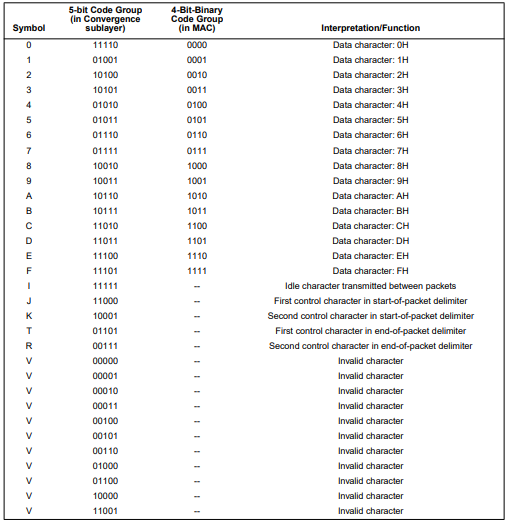
\includegraphics[width=0.45\textwidth]{tablica.png}
    \caption{Kodowane symbole kodu 4B5B}
    \label{fig:mojobrazek1}
\end{figure}

\subsubsection{Siatki Karnaugh}
\begin{figure}[H]  
    \centering
    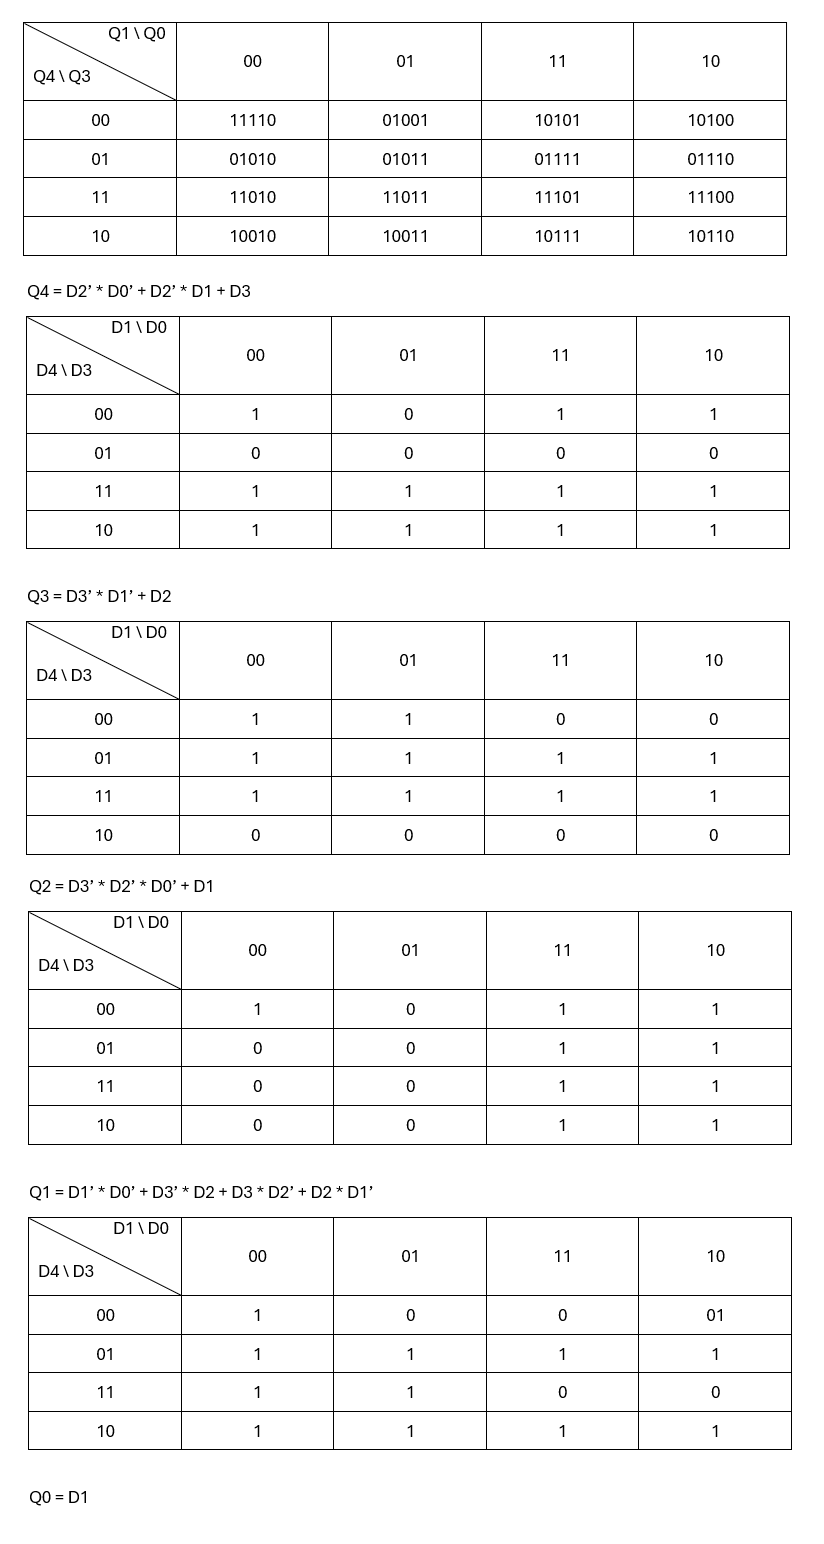
\includegraphics[width=0.8\textwidth]{siatki.png}
    \caption{Tablica prawdy przetłumaczona na siatki Karnaugh}
    \label{fig:mojobrazek2}
\end{figure}

\subsubsection{Uproszczony schemat kodera firmy Actel}
\begin{figure}[H]  
    \centering
    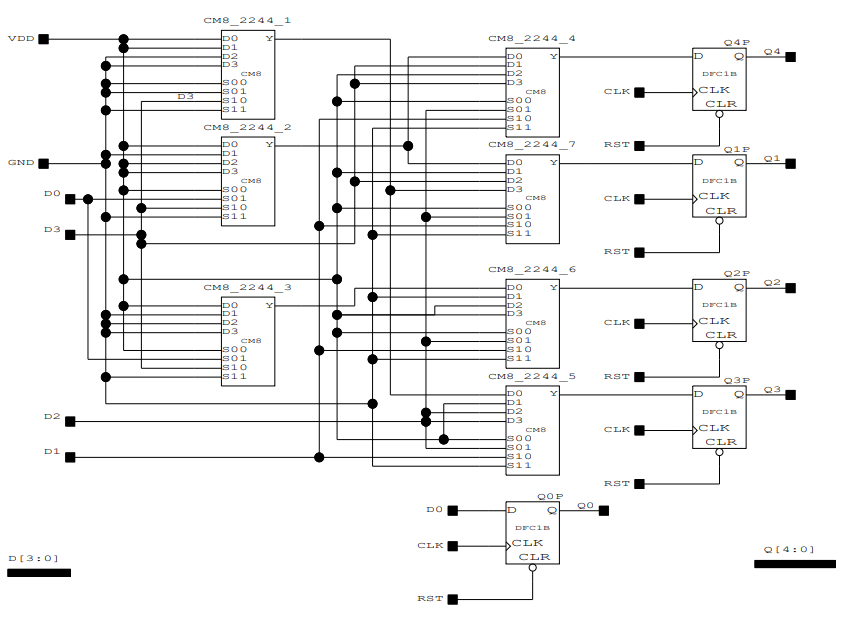
\includegraphics[width=0.8\textwidth]{fpga-4b5b.png}
    \caption{Uproszczony schemat kodera przy użyciu widoku logiki FPGA}
    \label{fig:mojobrazek2}
\end{figure}

\subsubsection{Opis kodera 4B5B przy użyciu PALASM2}
\begin{figure}[H]  
    \centering
    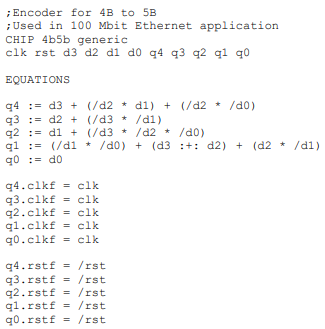
\includegraphics[width=0.6\textwidth]{palasm2.png}
    \caption{Schemat kodera 4B5B w języku PALASM2}
    \label{fig:mojobrazek3}
\end{figure}

\newpage

\subsection{Realizacja przy użyciu środowiska LTSpice}
\subsubsection{Wstęp}
\begin{itemize}
\item Na podstawie równań logicznych, uzyskanych dzięki zastosowaniu metody siatek Karnaugh, zbudowano układ składający się z czterech modułów kodujących, oznaczonych jako Q1, Q2, Q3 i Q4 [rys. 5]. Każdy z tych modułów odpowiedzialny jest za kodowanie poszczególnych symboli wyjściowych na podstawie bitów wejściowych [rys. 6-9].

\item Specyfikacja bitu Q0 jest bezpośrednio powiązana z bitem wejściowym D1, co wynika z zasady działania kodu 4B5B, gdzie bit Q0 replikuje wartość bitu D1. Taka zależność ma kluczowe znaczenie dla zachowania odpowiedniej struktury danych wyjściowych, która jest wymagana przez standard kodowania.

\item Dodatkowo, implementacja układu uwzględnia cztery źródła napięcia, oznaczone jako V1, V2, V3 oraz V4. Każde z tych źródeł napięcia zostało szczegółowo zdefiniowane i opisane, a ich role polegają na dostarczeniu odpowiedniego strumienia bitowego, który jest niezbędny dla poprawnego działania poszczególnych bloków kodujących.
\end{itemize}

\subsubsection{Realizacja schematu kodera w symulatorze LTSpice}
\begin{figure}[H]
    \centering
    \begin{adjustbox}{center}
        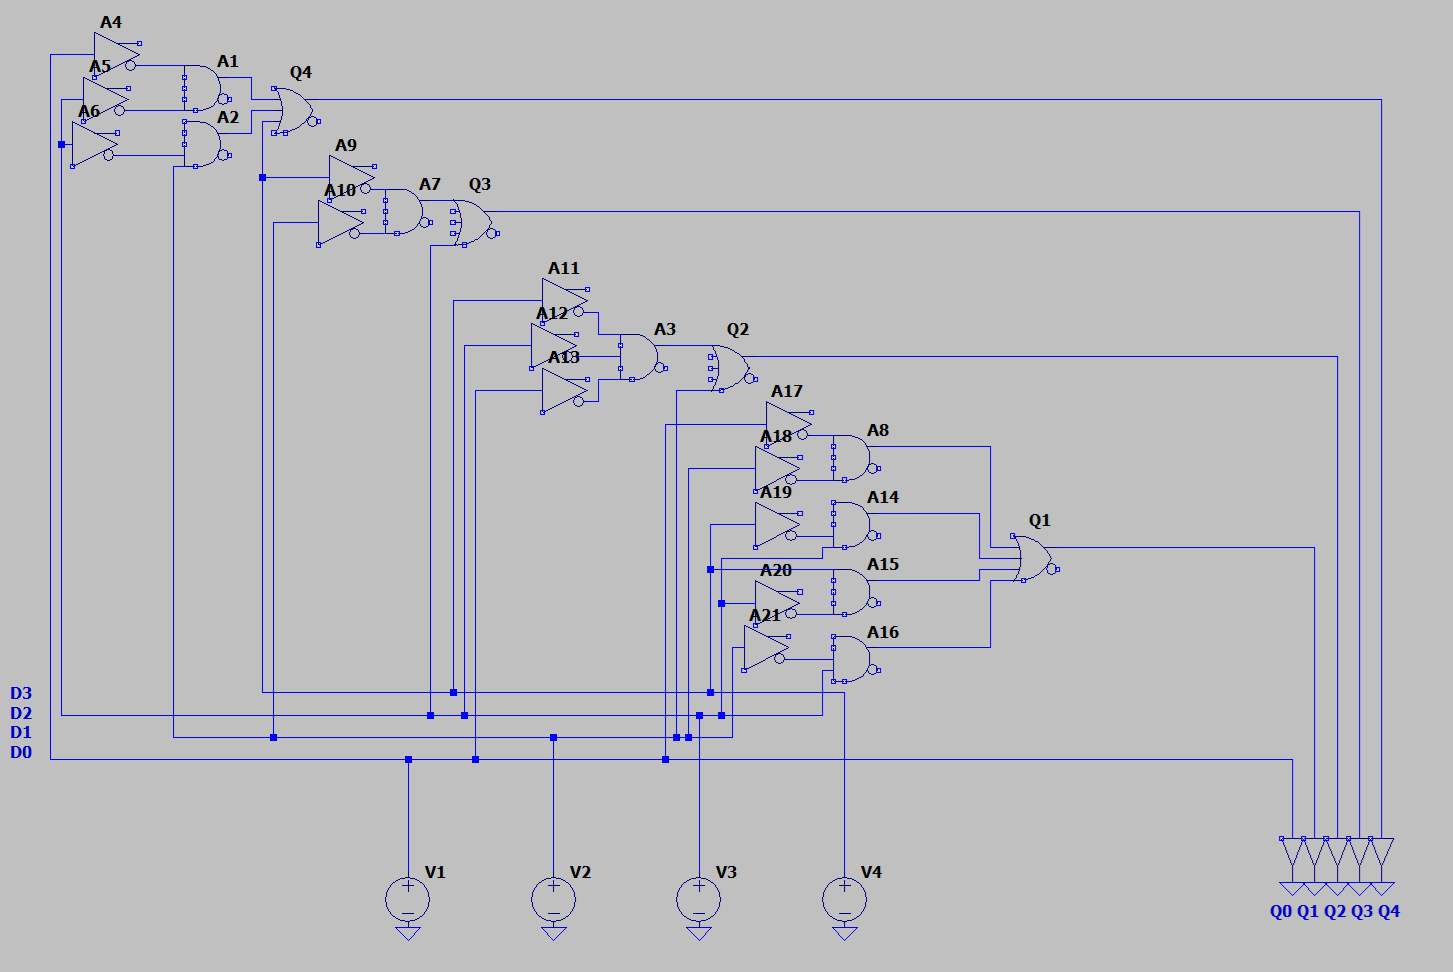
\includegraphics[width=1\textwidth]{ltspice-4b5b.png}
    \end{adjustbox}
    \caption{Realizacja schematu kodera w symulatorze LTSpice}
    \label{fig:mojobrazek}
\end{figure}

\subsubsection{Koder bitu Q1}
\begin{figure}[H]
    \centering
    \begin{adjustbox}{center}
        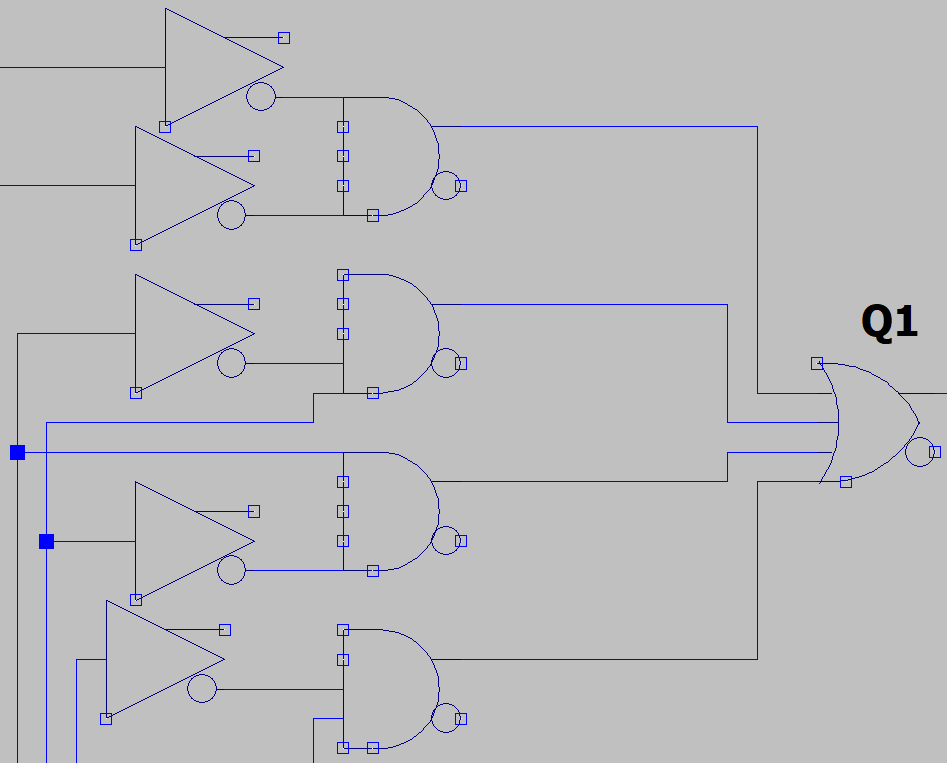
\includegraphics[width=0.85\textwidth]{q1.png}
    \end{adjustbox}
    \caption{Schemat częściowy kodera bitu Q1 w środowisku LTSpice}
    \label{fig:mojobrazek}
\end{figure}

\subsubsection{Koder bitu Q2}
\begin{figure}[H]
    \centering
    \begin{adjustbox}{center}
        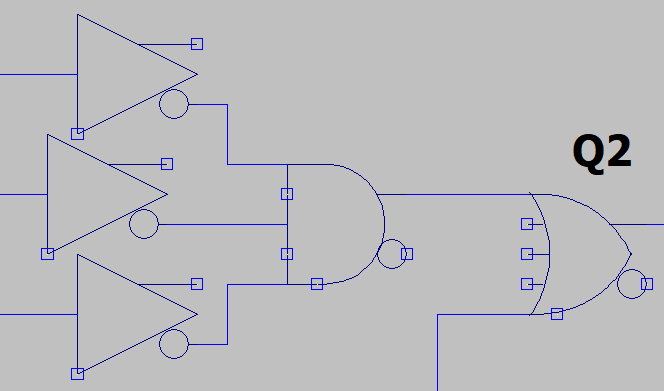
\includegraphics[width=0.8\textwidth]{q2.png}
    \end{adjustbox}
    \caption{Schemat częściowy kodera bitu Q2 w środowisku LTSpice}
    \label{fig:mojobrazek}
\end{figure}

\subsubsection{Koder bitu Q3}
\begin{figure}[H]
    \centering
    \begin{adjustbox}{center}
        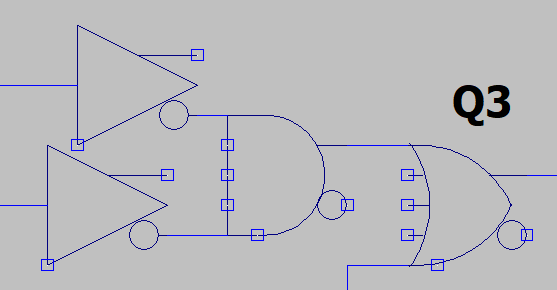
\includegraphics[width=1\textwidth]{q3.png}
    \end{adjustbox}
    \caption{Schemat częściowy kodera bitu Q3 w środowisku LTSpice}
    \label{fig:mojobrazek}
\end{figure}

\subsubsection{Koder bitu Q4}
\begin{figure}[H]
    \centering
    \begin{adjustbox}{center}
        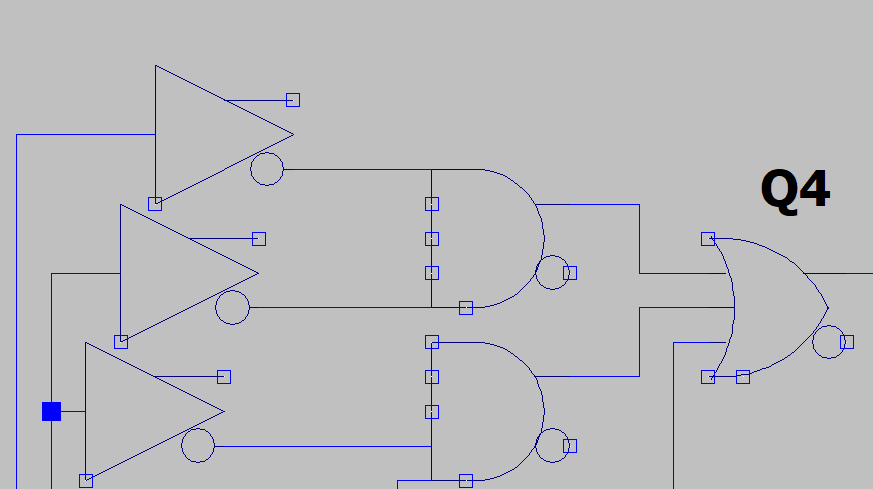
\includegraphics[width=1\textwidth]{q4.png}
    \end{adjustbox}
    \caption{Schemat częściowy kodera bitu Q4 w środowisku LTSpice}
    \label{fig:mojobrazek}
\end{figure}
\newpage

\subsection{Symulacja działania kodera}
\subsubsection{Wstęp}
\begin{itemize}
\item W ramach symulacji źródła sygnału pseudolosowego, wykorzystano źródła napięcia V1, V2, V3 oraz V4. Program symulacyjny LTSpice daje możliwość zastosowania źródła napięcia typu PWL, które jest definiowane w pliku tekstowym, co pozwala na odwzorowanie warunków operacyjnych.

\item W symulacji, każde z tych źródeł napięcia skonfigurowano do generowania sekwencji napięciowej, która odpowiada sekwencjom sygnałów danych binarnych. Źródło napięcia zmienia stan w określonych momentach czasowych: w chwili 5 ns napięcie jest równe 0 V, natomiast w chwili 5.1 ns wzrasta do 5 V, i tak dalej, aż do chwili 20 ns generując sygnał prostokątny. Taka sekwencja napięciowa jest szczegółowo przedstawiona na [rys. 10] oraz opisana w [tab. 1]. Czas trwania sygnału wybrano tak, aby spełniać założenia specyfikacyjne zegara według normy IEEE 802.3. \cite{ieee802}

\end{itemize}

\subsubsection{Zadany sygnał wejściowy}
\begin{figure}[ht]
    \centering
    \begin{adjustbox}{center}
        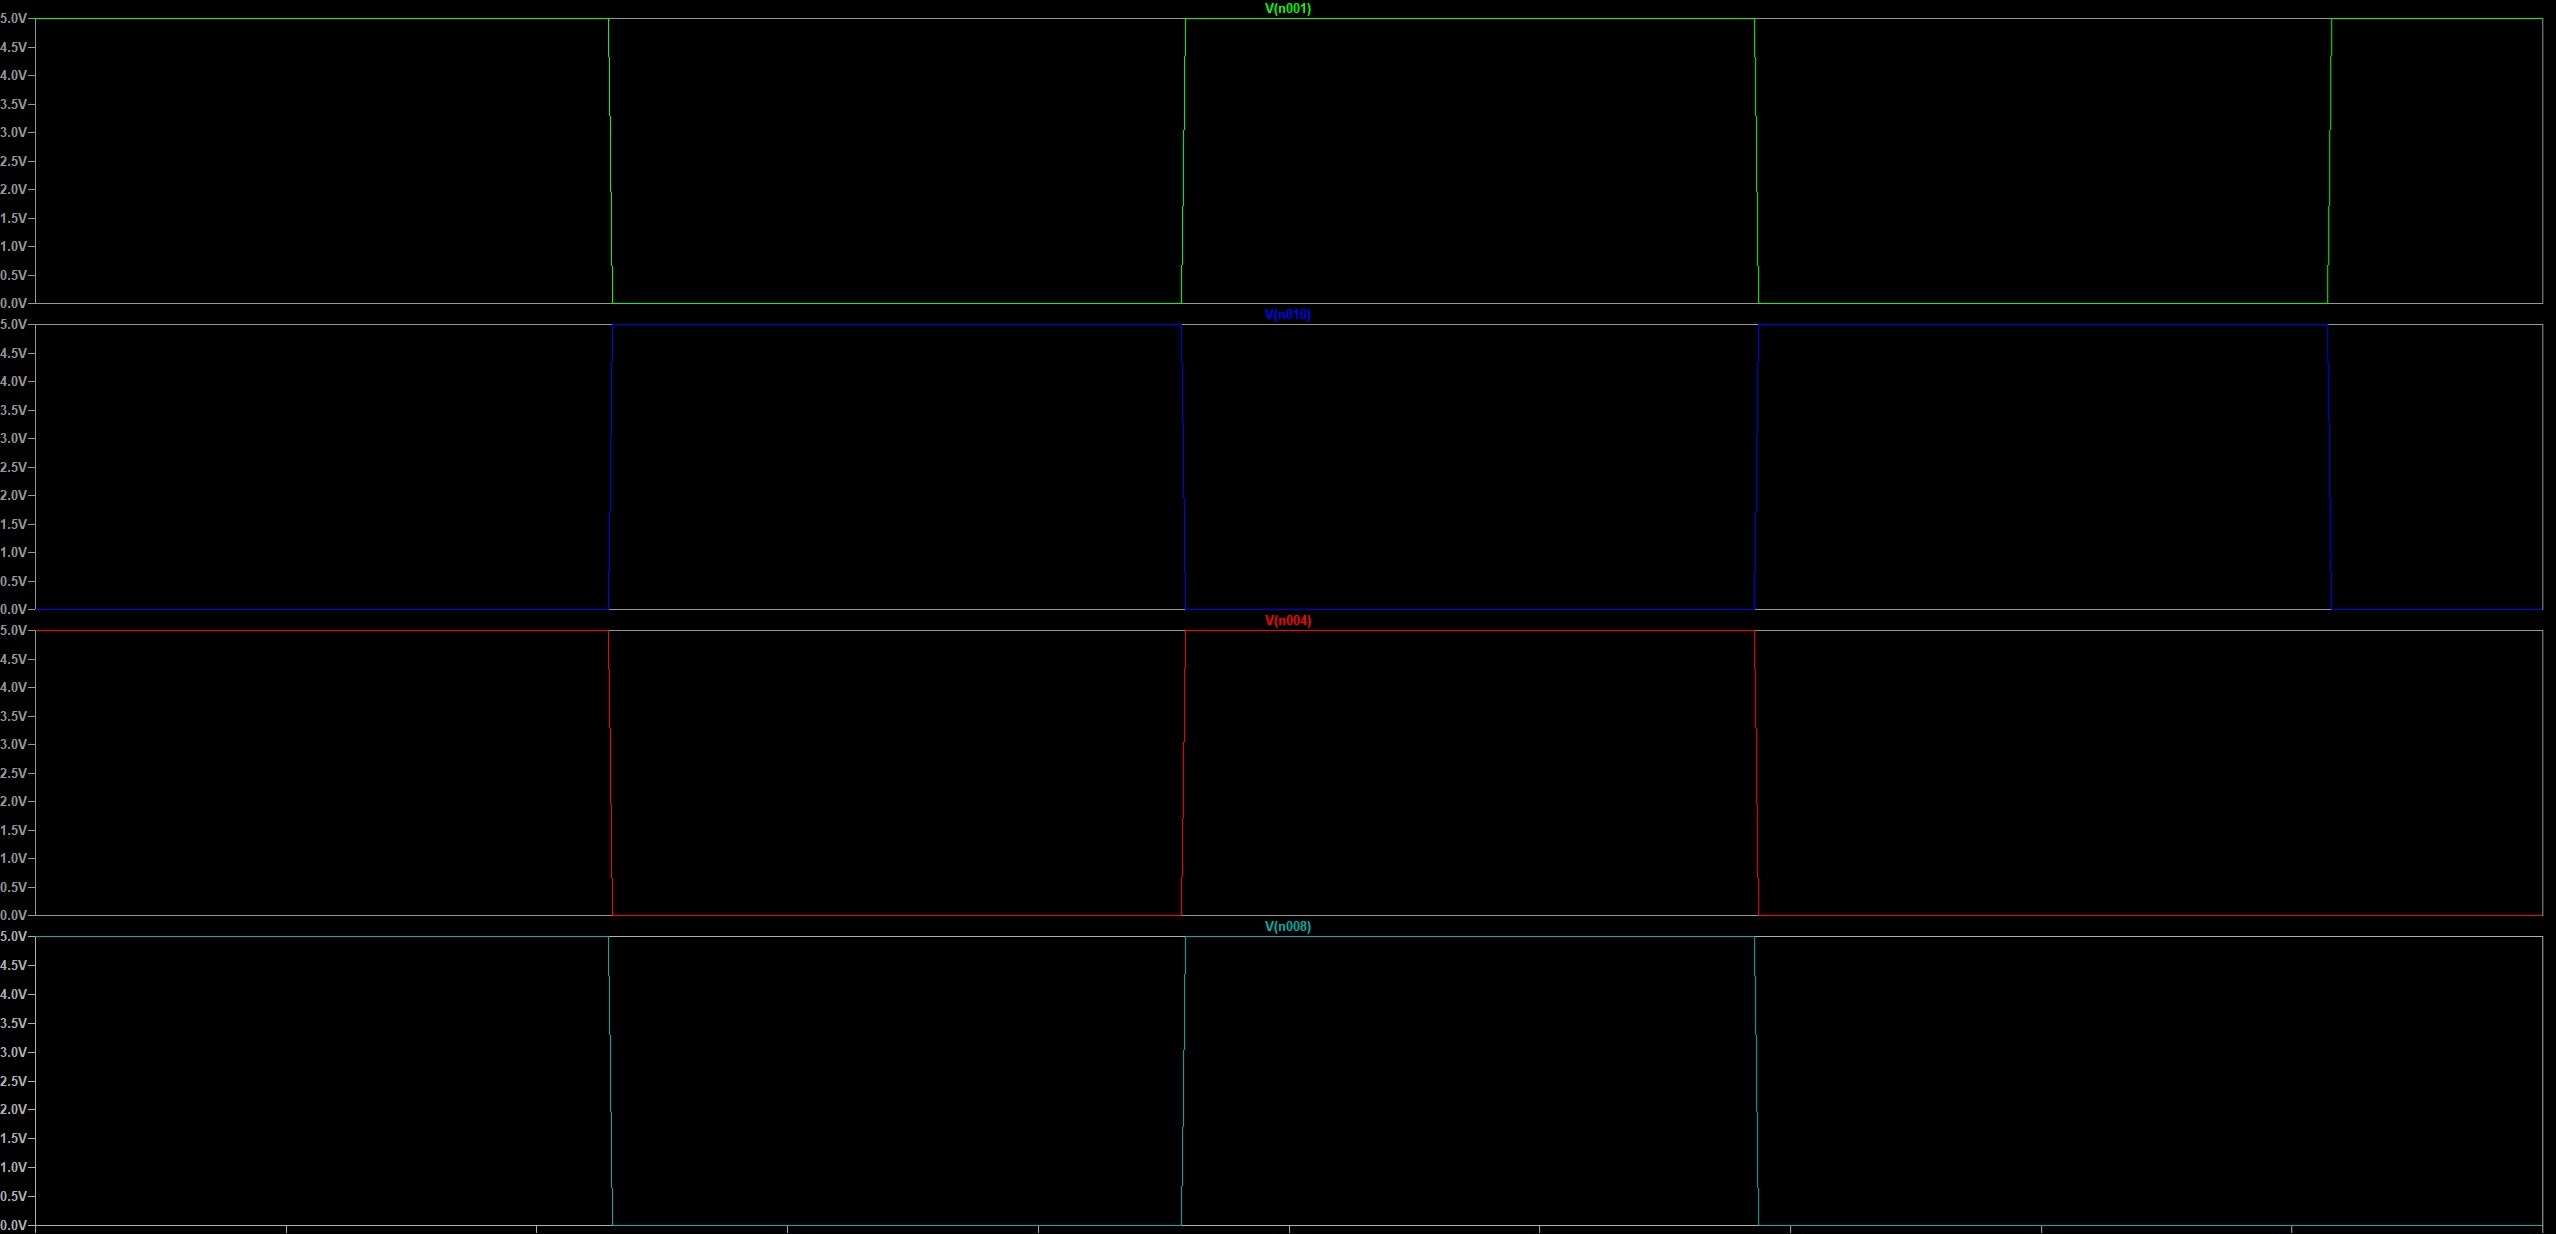
\includegraphics[width=0.70\textwidth]{wejsciowe.jpg}
    \end{adjustbox}
    \caption{Wykresy wejść bitów D0, D1, D2, D3}
    \label{fig:mojobrazek}
\end{figure}

\begin{table}[ht]
    \centering 
    \caption{Wymuszenia pseudolosowe na źródłach}
    \vspace{20pt} 
    \label{tab:tabela} 
    \begin{tabular}{|c|c|c|c|c|} 
    \hline 
   \textbf{Wejście D0} & \textbf{Wejście D1} & \textbf{Wejście D2} & \textbf{Wejście D3} \\ \hline % Nagłówki kolumn
    5 0 & 5 5 & 5 5 & 5 \\ \hline % Dane w pierwszym wierszu
    5.1n 5 & 5.1n 0 & 5.1n 0 & 5.1n 0 \\ \hline % Dane w drugim wierszu
    10n 5 & 10n 0 & 10n 0 & 10n 0\\ \hline % Dane w drugim wierszu
    10.1n 0 & 10.1n 5 & 10.1n 5 & 10.1n 5 \\ \hline % Dane w drugim wierszu
    20n 0 & 20n 5 & 20n 5 & 20n 5 \\ \hline % Dane w drugim wierszu
    20.1n 5 & 20.1n 5 & 20.1n 0 & 20.1n 0 \\ \hline % Dane w drugim wierszu
    Symbol: 1010 & Symbol: 0101 & Symbol: 1010 & Symbol: 0101 \\ \hline % Dane w drugim wierszu
    \end{tabular}
    \end{table}

\newpage

\subsubsection{Sygnał wyjściowy}
\begin{figure}[ht]
    \centering
    \begin{adjustbox}{center}
        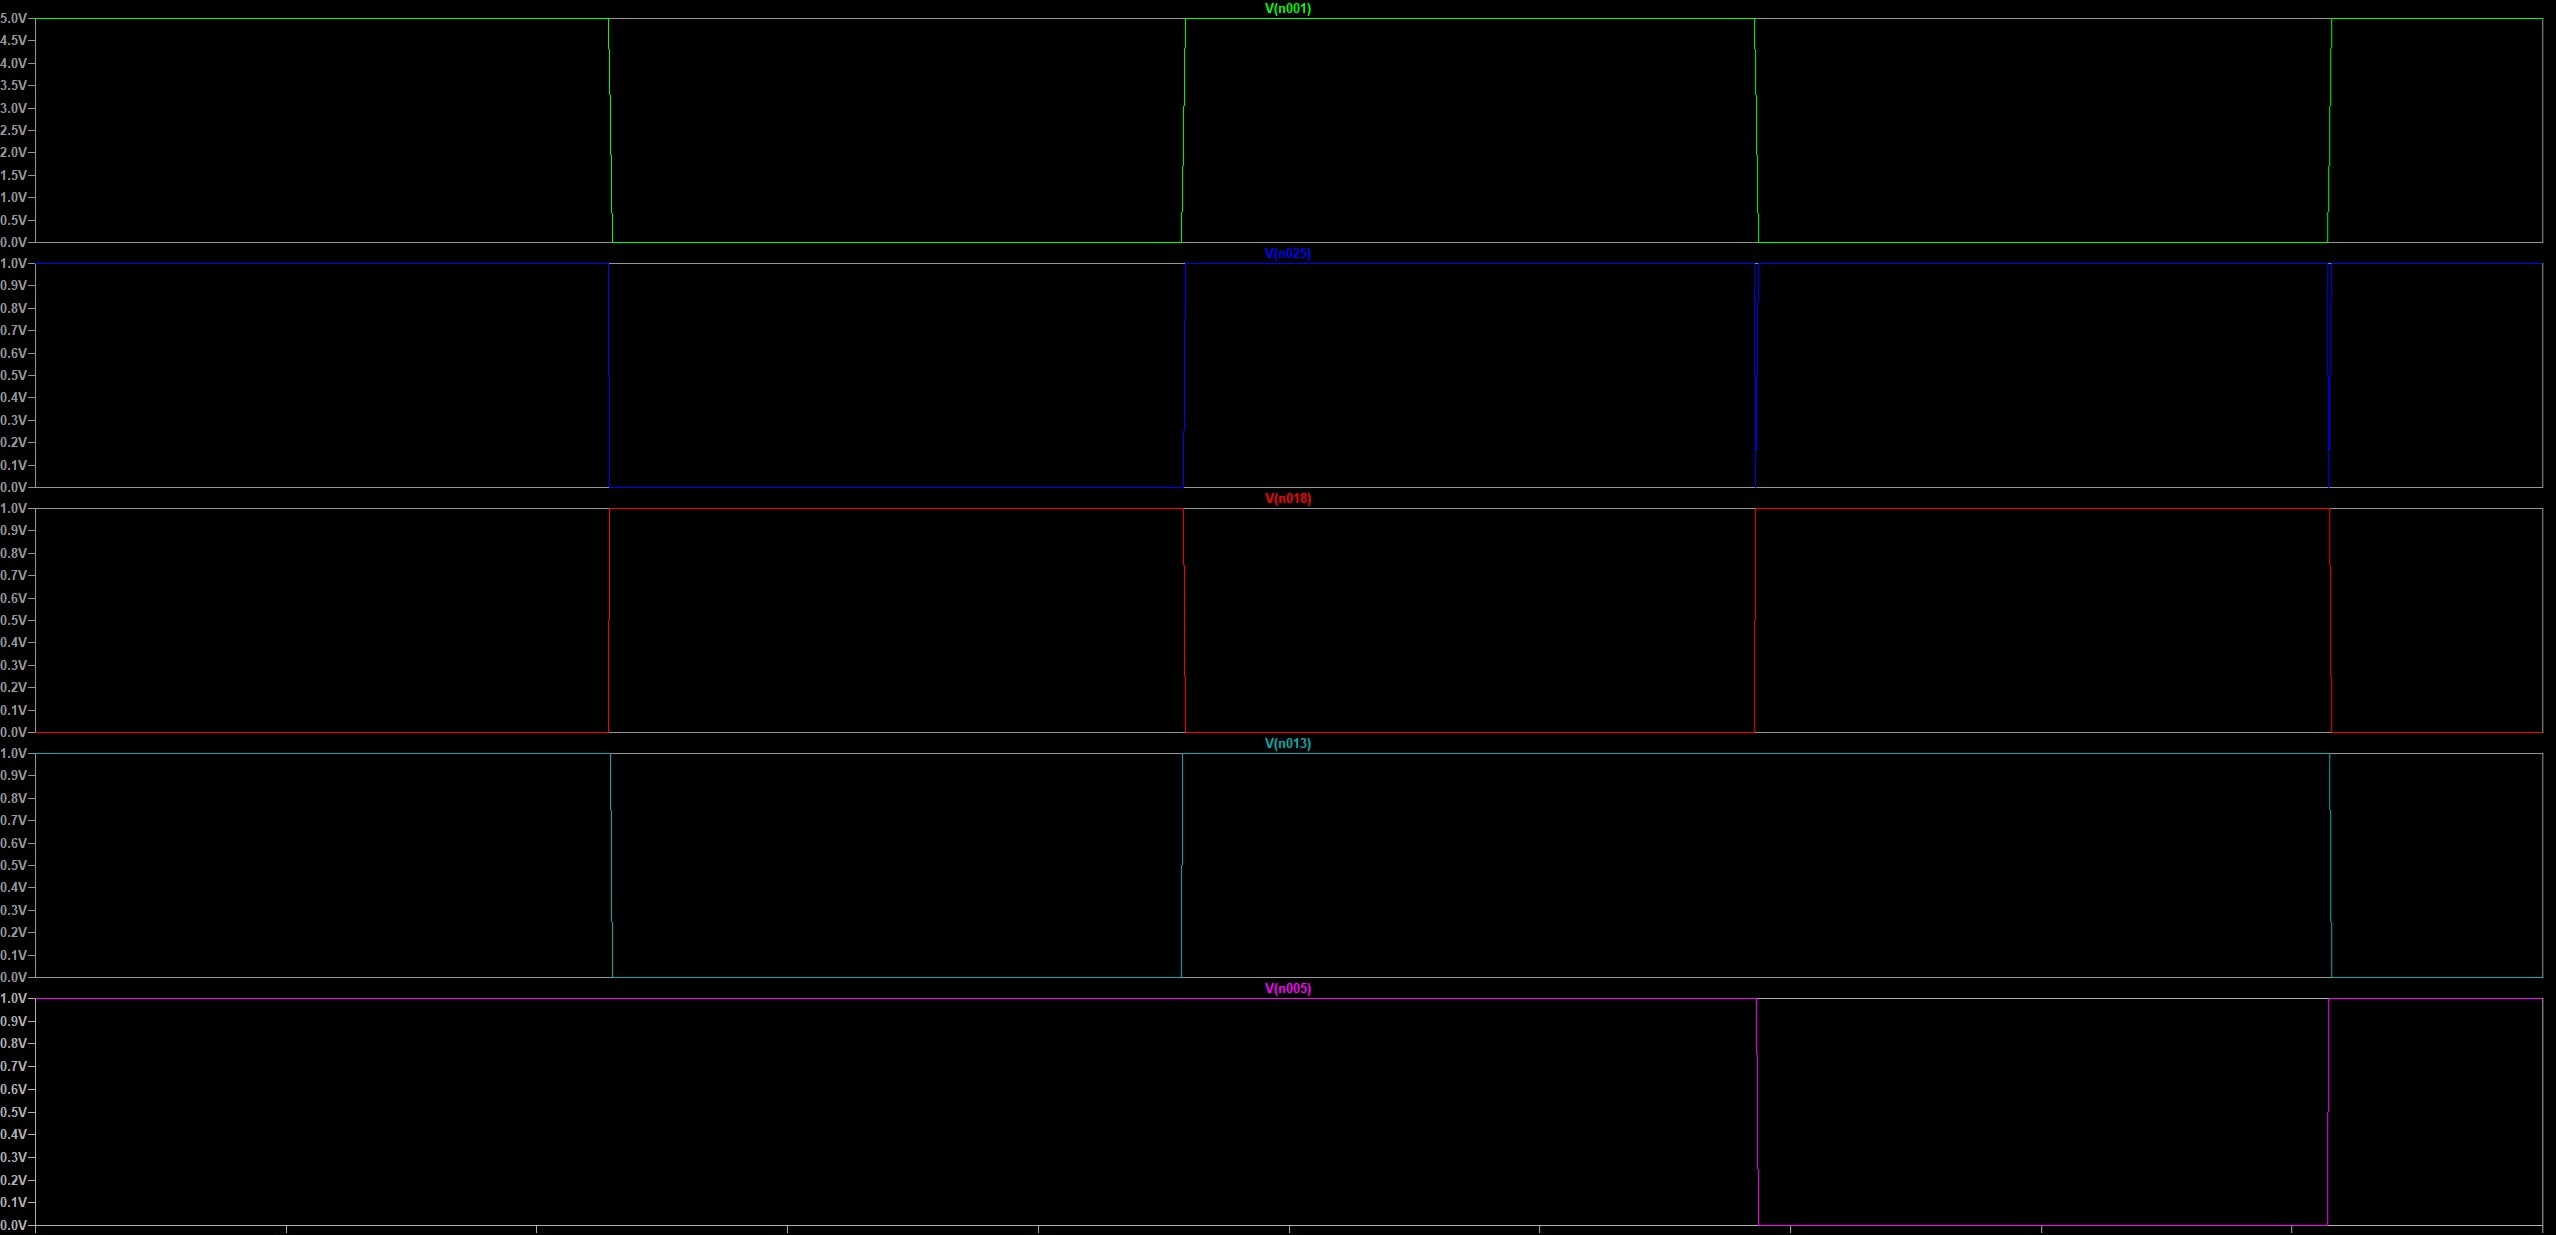
\includegraphics[width=1.3\textwidth]{wyjsciowe.jpg}
    \end{adjustbox}
    \caption{Wykresy wyjść bitów Q0, Q1, Q2, Q3, Q4}
    \label{fig:mojobrazek}
\end{figure}

\begin{table}[ht]
    \centering 
    \caption{Zakodowane symbole 4B5B}
    \vspace{20pt} 
    \label{tab:tabela} 
    \begin{tabular}{|c|c|c|c|c|c|} 
    \hline 
    \textbf{Lp.} & \textbf{Wyjście Q0} & \textbf{Wyjście Q1} & \textbf{Wyjście Q2} & \textbf{Wyjście Q3} & \textbf{Wyjście Q4} \\ \hline 
    Symbol 1 & 1 & 1 & 0 & 1 & 1 \\ \hline 
    Symbol 2 & 0 & 0 & 1 & 0 & 1 \\ \hline 
    Symbol 3 & 1 & 1 & 0 & 1 & 1 \\ \hline 
    Symbol 4 & 0 & 1 & 1 & 1 & 0 \\ \hline 
    \end{tabular}
\end{table}

\newpage

\subsection {Analiza uzyskanych wyników}
\subsubsection {Wstęp}
W odniesieniu do układu referencyjnego, przebiegi sygnałów wygenerowane przez analizowany koder wykazują identyczność stanów, co umożliwia potwierdzenie poprawności działania układu kodującego. Dokładna analiza stanów, przedstawionych w symulacji za pomocą oprogramowania LTSpice, pozwala na obserwację zgodności wyników uzyskanych (prezentowanych na rysunku 11) z oczekiwanymi rezultatami, które zostały szczegółowo określone w tabeli 2.
\subsubsection {Wnioski}
\begin{itemize}
\item W trakcie projektu zrealizowanego na elementach idealnych nie napotkano znaczących przeszkód, co stanowi dowód na efektywne wykorzystanie środowiska LTSpice do modelowania i analizy układów elektronicznych. Proces ten nie tylko wzmocnił nasze umiejętności w zakresie korzystania z tego narzędzia, ale także nauczył nas efektywnego poszukiwania specjalistycznych informacji, które często były trudno dostępne w dostępnych źródłach internetowych.
\item Długotrwała analiza dostępnych materiałów pozwoliła na głębsze zrozumienie problemu oraz wypracowanie odpowiednich rozwiązań. Finalnie, po przeprowadzeniu szeregu testów i weryfikacji, koder został skutecznie zaimplementowany i zademonstrował prawidłowe działanie zgodnie z oczekiwaniami. Wynik ten nie tylko potwierdza skuteczność naszego podejścia projektowego, ale także podkreśla wartość dogłębnej analizy teoretycznej i praktycznej w procesie inżynierskim.
\end{itemize}

%%%%%%%%%%%%
%5. Realizacja schematu kodera przy użyciu elementów rzeczywistych
%%%%%%%%%%%%

\newpage
\section{Realizacja schematu kodera przy użyciu elementów rzeczywistych}
\subsection{Wstęp}
\begin{itemize}
    \item 
    Realizacja schematu kodera z wykorzystaniem elementów rzeczywistych przebiegła z napotkaniem pewne wyzwań związanych z dostępnością tych komponentów w środowisku LTSpice. Standardowa biblioteka LTSpice nie zawierała wszystkich potrzebnych elementów rzeczywistych, co skłoniło nas do poszukiwania zewnętrznych źródeł. Ostatecznie, niezbędne komponenty udało się uzyskać dzięki plikom dostępnym na amatorskiej encyklopedii wiedzy o środowisku LTSpice. \cite{ltwiki} \cite{borod}
    \item 
    Po pobraniu odpowiednich plików, przystąpiono do modyfikacji pierwotnego schematu, który opierał się na elementach idealnych. Zamieniono te elementy na ich rzeczywiste odpowiedniki, co wymagało dostosowania parametrów układu. Zmiana ta pozwoliła na osiągnięcie realistycznej symulacji, co jest kluczowe dla weryfikacji działania kodera w realnych warunkach. Pomimo początkowych trudności, adaptacja układu do warunków zbliżonych do rzeczywistych przebiegła poprawnie. \cite{actel}
    
\end{itemize}

\subsection{Skrócona specyfikacja techniczna elementów}
\begin{itemize}
    \item \textbf{Inwertery NOT 74HC04}\newline 
    Czas narastania i opadania sygnału: Typowo 6 ns przy obciążeniu 50 pF. \cite{hc04}
    
    \item \textbf{Bramki AND 74HC08}\newline 
    Czas narastania i opadania sygnału: Około 8 ns przy obciążeniu 50 pF. \cite{hc08}

    \item \textbf{Bramki OR 74HC32}\newline 
    Czas narastania i opadania sygnału: Osiąga do 7 ns przy obciążeniu 50 pF. \cite{hc32}

    \item \textbf{Bramka AND 74HC11}\newline 
    Czas narastania i opadania sygnału: Zazwyczaj wynosi około 9 ns przy obciążeniu 50 pF. \cite{hc11}

\end{itemize}

\newpage
\subsection{Realizacja w środowisku LTSpice} 
\subsubsection{Wstęp}
\begin{itemize}
    \item 
    Realizacja schematu kodera na elementach rzeczywistych wiązała się z koniecznością zamiany elementów idealnych, standardowo dostępnych w bibliotece LTSpice, na ich rzeczywiste odpowiedniki. Elementy te to 74HC04, 74HC08, 74HC32, i 74HC11. \cite{hc04} \cite{hc08} \cite{hc32} \cite{hc11} Modeli tych nie znaleziono w standardowych bibliotekach LTSpice, niezbędne komponenty udało się uzyskać dzięki plikom dostępnym na amatorskiej encyklopedii wiedzy o środowisku LTSpice.  \cite{ltwiki} \cite{borod}
    \item 
    Przeprwadzono proces integracji tych modeli z istniejącym schematem kodera. Wymagało to modyfikacji parametrów komponentów w schemacie oraz dostosowania połączeń, aby uwzględnić rzeczywiste charakterystyki czasowe i fizyczne komponentów. Dzięki tym zmianom, udało się osiągnąć wiarygodne rezultaty symulacji, co pozwoliło na ocenę działania kodera w warunkach, występują podczas rzeczywistego użytkowania.
\end{itemize}

\subsubsection{Realizacja kodera}
\begin{figure}[H]
    \centering
    \begin{adjustbox}{center}
        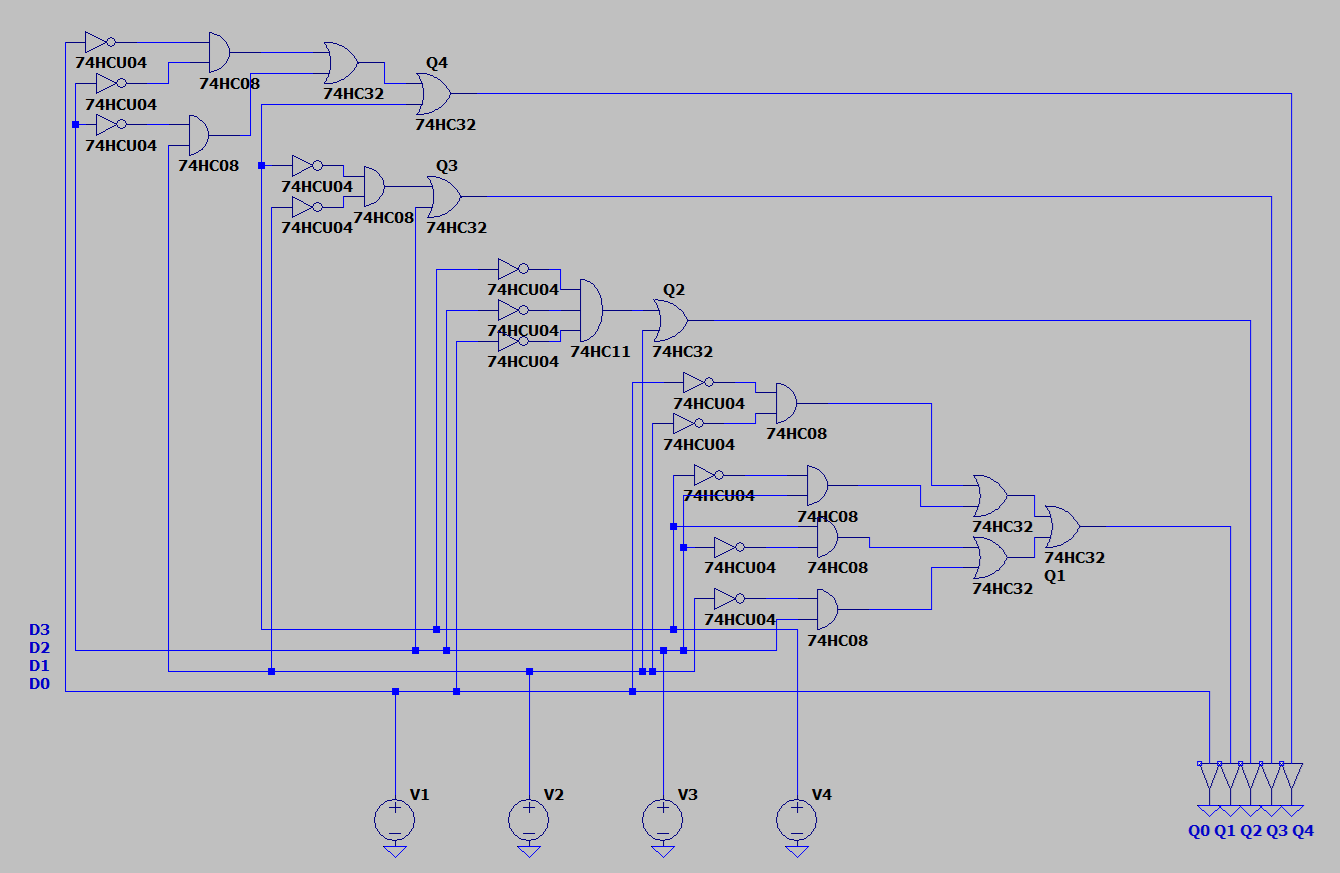
\includegraphics[width=1.1\textwidth]{ltspice-rzeczywiste.png}
    \end{adjustbox}
    \caption{Realizacja schematu kodera w środowisku LTSpice}
    \label{fig:mojobrazek}
\end{figure}
\subsubsection{Koder bitu Q1}
\begin{figure}[H]
    \centering
    \begin{adjustbox}{center}
        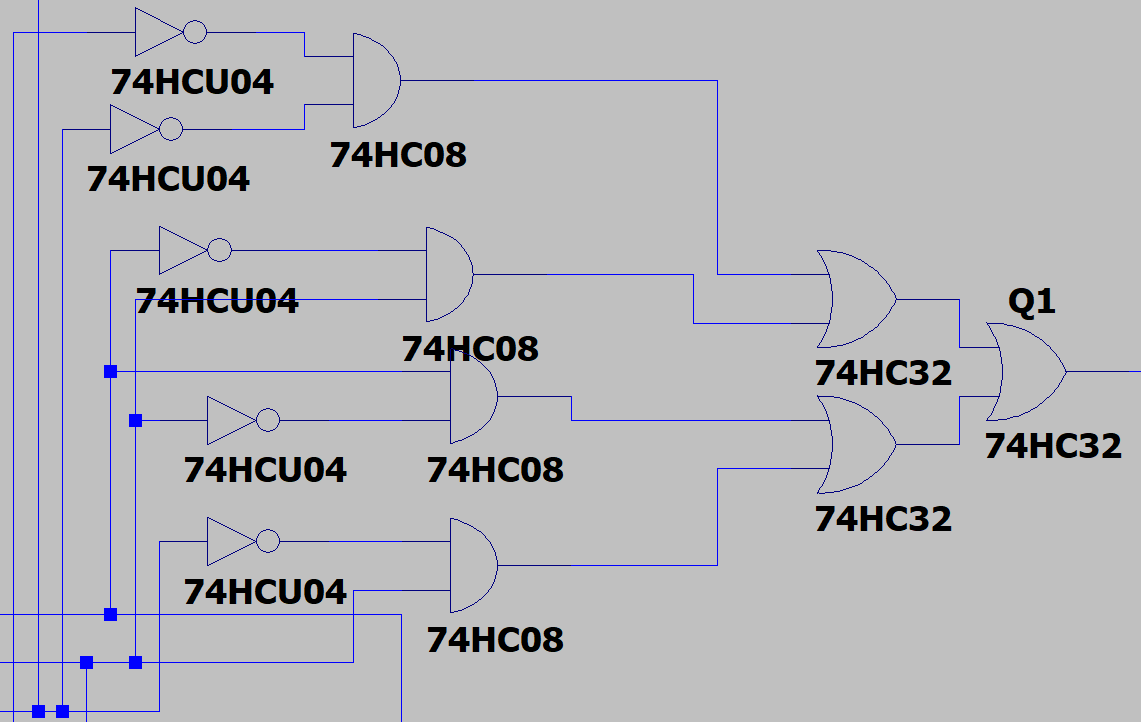
\includegraphics[width=0.9\textwidth]{q1-r.png}
    \end{adjustbox}
    \caption{Schemat częściowy kodera bitu Q1 w środowisku LTSpice}
    \label{fig:mojobrazek}
\end{figure}
\subsubsection{Koder bitu Q2}
\begin{figure}[H]
    \centering
    \begin{adjustbox}{center}
        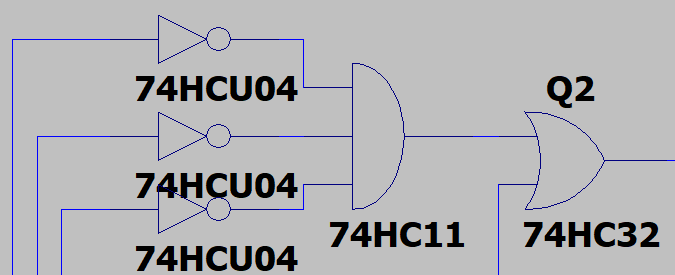
\includegraphics[width=0.9\textwidth]{q2-r.png}
    \end{adjustbox}
    \caption{Schemat częściowy kodera bitu Q2 w środowisku LTSpice}
    \label{fig:mojobrazek}
\end{figure}
\subsubsection{Koder bitu Q3}
\begin{figure}[H]
    \centering
    \begin{adjustbox}{center}
        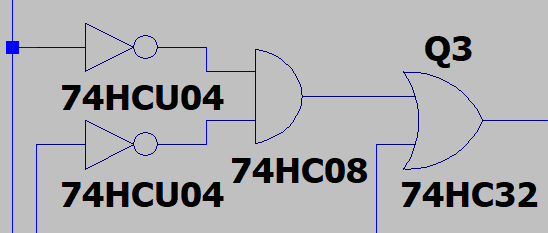
\includegraphics[width=0.9\textwidth]{q3-r.png}
    \end{adjustbox}
    \caption{Schemat częściowy kodera bitu Q3 w środowisku LTSpice}
    \label{fig:mojobrazek}
\end{figure}
\subsubsection{Koder bitu Q4}
\begin{figure}[H]
    \centering
    \begin{adjustbox}{center}
        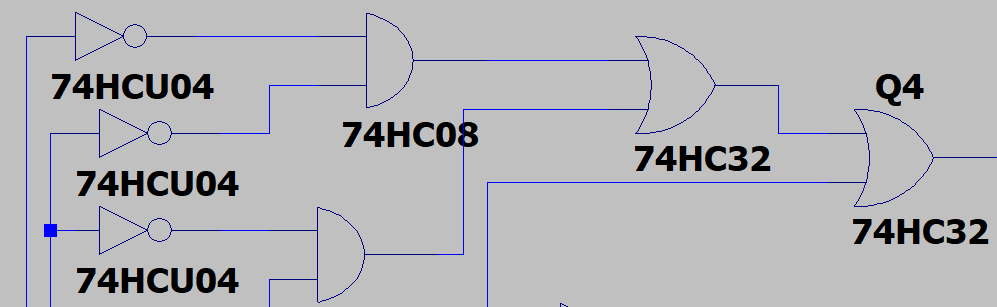
\includegraphics[width=0.9\textwidth]{q4-r.png}
    \end{adjustbox}
    \caption{Schemat częściowy kodera bitu Q4 w środowisku LTSpice}
    \label{fig:mojobrazek}
\end{figure}
\newpage
\subsection{Symulacja działania}
\subsubsection{Wstęp}
\begin{itemize}
    \item Analogicznie do przypadku układu na elementach idealnych użylismy źródeł pseudolosowych, tutaj źródło sygnału danych zostało przedłużone aby działać do 500ns. Wykorzystywane są źródła napięcia V1, V2, V3 oraz V4. 
    Wycinek definicji działania przedstawiona jest w załączonym pliku
    tekstowym, co pozwala na precyzyjne odwzorowanie rzeczywistych warunków operacyjnych
    \item W symulacji, każde z tych źródeł napięcia zostało skonfigurowane do generowania sekwencji napięciowej, która odpowiada sekwencjom zegarowych sygnałów binarnych. Analogicznie jak w układzie na elementach idealnych, źródło napięcia zmienia stan w  określonych momentach czasowych: w chwili 5 ns napięcie jest równe 0 V, natomiast w chwili 5.1 ns wzrasta do 5 V, i tak dalej, aż do chwili 500 ns generując sygnał prostokątny. Taka sekwencja napięciowa jest w wycinku przedstawiona na [rys. 17]. Czas trwania sygnału wybrano tak, aby spełniać założenia specyfikacyjne zegara według normy IEEE 802.3. \cite{ieee802}
\end{itemize} 

\subsubsection{Zadany sygnał wejściowy}
\begin{figure}[ht]
    \centering
    \begin{adjustbox}{center}
        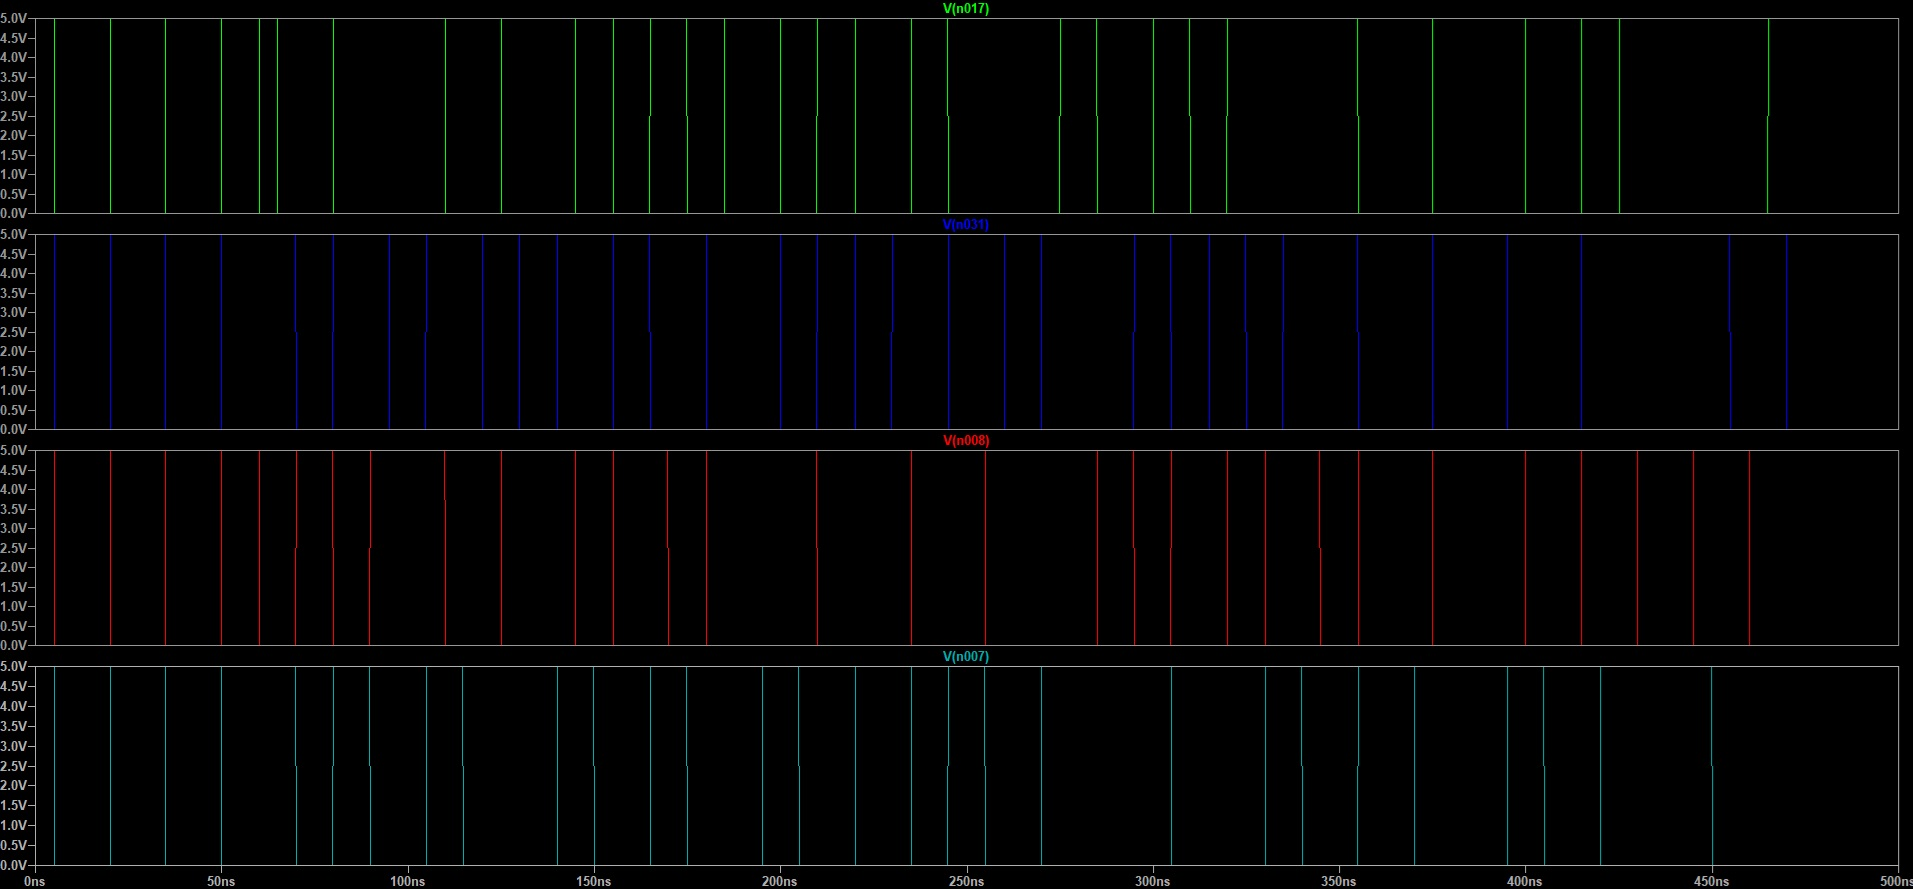
\includegraphics[width=1.4\textwidth]{wejsciowe-rzecz.jpg}
    \end{adjustbox}
    \caption{Wykresy wejść bitów D0, D1, D2, D3}
    \label{fig:mojobrazek}
\end{figure}

\newpage

\subsubsection{Sygnał wyjściowy}
\begin{figure}[ht]
    \centering
    \begin{adjustbox}{center}
        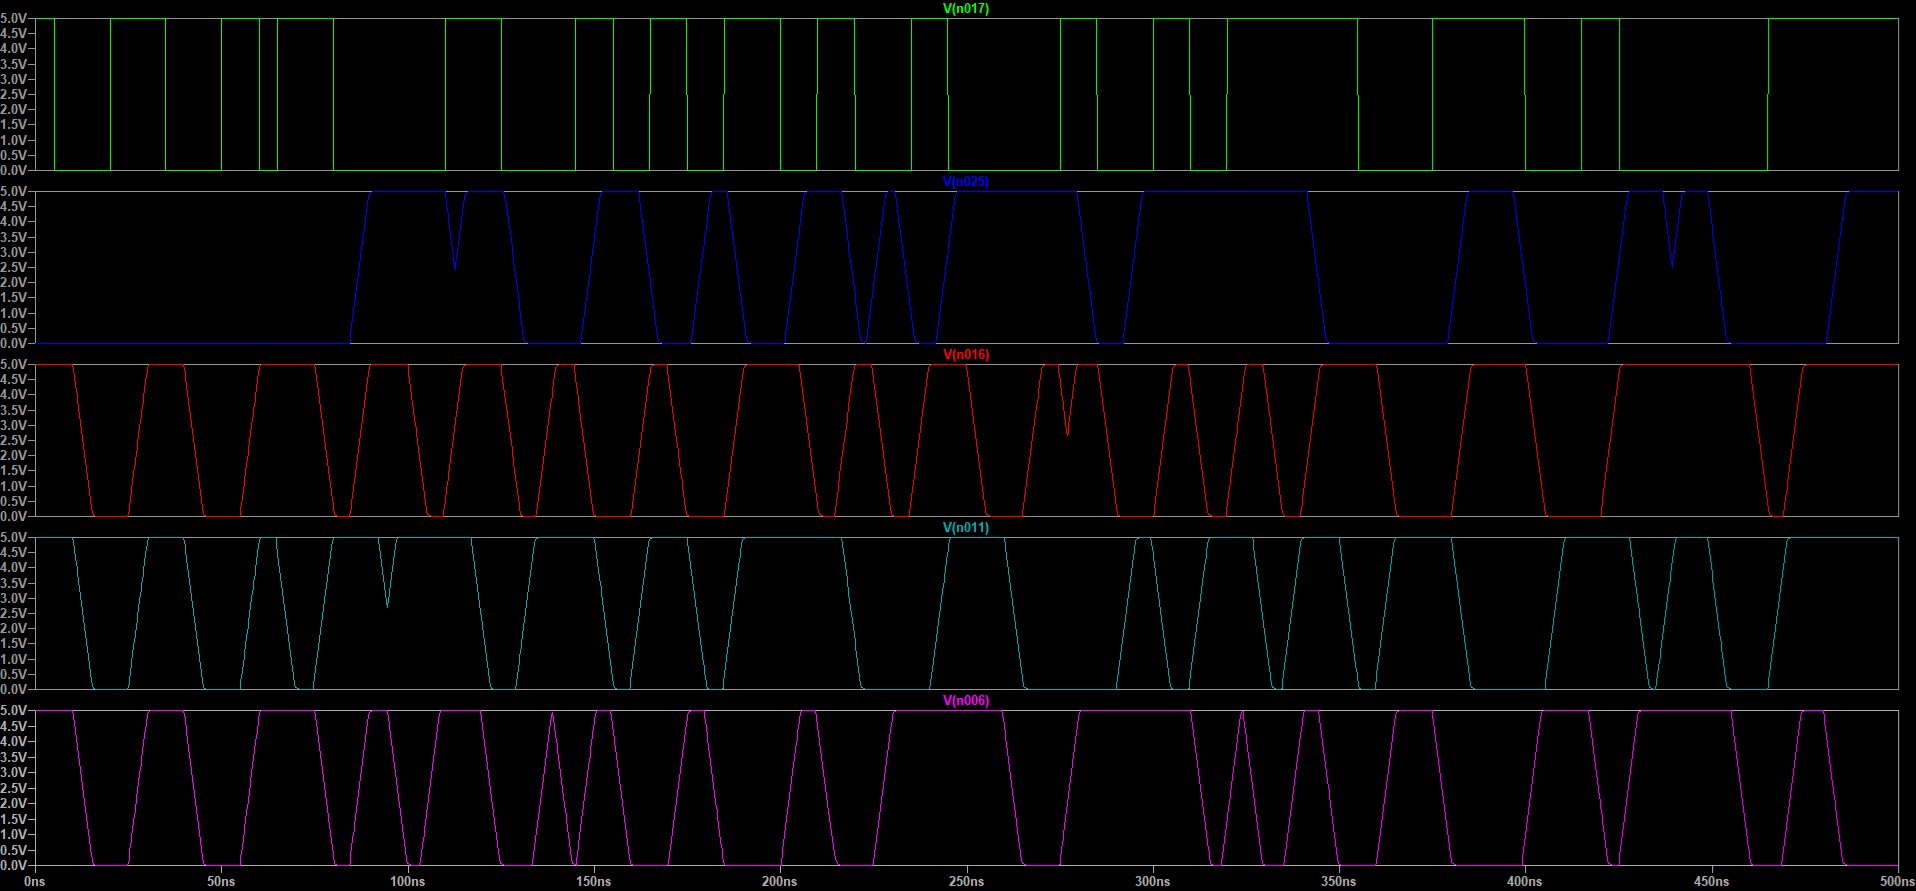
\includegraphics[width=1.45\textwidth]{wyjsciowe-rzecz.png}
    \end{adjustbox}
    \caption{Wykresy wyjść bitów Q0, Q1, Q2, Q3, Q4}
    \label{fig:mojobrazek}
\end{figure}

\newpage

\subsection {Analiza uzyskanych wyników}
\subsubsection {Wstęp}
\begin{itemize}
\item W ramach projektu zrealizowano symulację kodera wykorzystując zarówno elementy idealne, jak i rzeczywiste, w środowisku LTSpice. Z analizy wyników symulacji, której efekty są widoczne na załączonym obrazie, można zaobserwować znaczące różnice w zachowaniu sygnałów generowanych przez te dwa rodzaje elementów. Głównym celem symulacji było porównanie dynamiki sygnałów wyjściowych kodera z uwzględnieniem czasów narastania i opadania, które są kluczowe w zastosowaniach rzeczywistych.

\item Symulacja na elementach rzeczywistych pokazała wyraźne efekty ograniczeń fizycznych komponentów, takich jak artefakty sygnału, czas narastania i opadania sygnału, co nie występuje w przypadku modeli idealnych. Te różnice mają krytyczne znaczenie dla projektowania układów cyfrowych, które działają w rzeczywistych warunkach, zapewniając dokładność w dostarczaniu danych.
\end{itemize}

\subsubsection {Parametry układu}
\begin{itemize}
\item \textbf{Przepustowość przy użyciu elementów idealnych}: \( 100Mbit/s \pm 1\% \)
\item \textbf{Czas narastania}: \( 5ns \pm 1\% \)
\item \textbf{Czas trwania bitu}: \( 10ns \pm 1\% \)
\item \textbf{Przybliżony czas trwania symbolu}: \( 15ns \pm 1\% \)
\item \textbf{Zmierzona przepustowość przy użyciu elementów rzeczywistych}:  \( 80Mbit/s \pm 10\% \)
\end{itemize}

\subsubsection {Wnioski}
\begin{itemize}
\item \textbf{Czasy Narastania i Opadania}: Symulacja z elementami rzeczywistymi uwidoczniła czasy narastania i opadania na sygnałach wyjściowych, które są nieobecne w symulacji z elementami idealnymi. Te czasy wpływają na synchronizację sygnału w rzeczywistych aplikacjach cyfrowych, gdzie dokładne czasowanie jest niezbędne. Tworząc układy należy brać pod uwagę te parametry, aby zapewnić niezawodność i efektywność działania układów w różnych warunkach operacyjnych.

\item \textbf{Optymalizacja}: Realizując układy, należy zwrócić szczególną uwagę na minimalizację ilości elementów, gdyż każdy zbędny, błędnie dobrany lub nieoptymalnie wykorzystany element generuje dodatkowe opóźnienia lub błędy kodowania, co bezpośrednio przekłada się na wyniki końcowe.
\newpage
\item \textbf{Artefakty}: Artefakty sygnału wskazują na to, że realne komponenty posiadają ograniczenia w szybkości reakcji na zmiany stanów, co jest kluczowe w szybkich systemach cyfrowych. Szybkość zmiany stanu sygnału wpływa na możliwość prawidłowego odczytu danych przez inne komponenty systemu. W obu przypadkach napięcie spada znacznie poniżej oczekiwanej wartości 5V, osiągając wartości około 2.4V i 2.7V. Tego rodzaju spadki mogą być wynikiem różnych czynników, takich jak opór wewnętrzny elementów lub nieidealne właściwości komponentów, które nie są w stanie utrzymać stabilnego poziomu napięcia pod obciążeniem.

\end{itemize}
\subsubsection{Artefakty sygnału}
\begin{figure}[ht]
    \centering
    \begin{adjustbox}{center}
        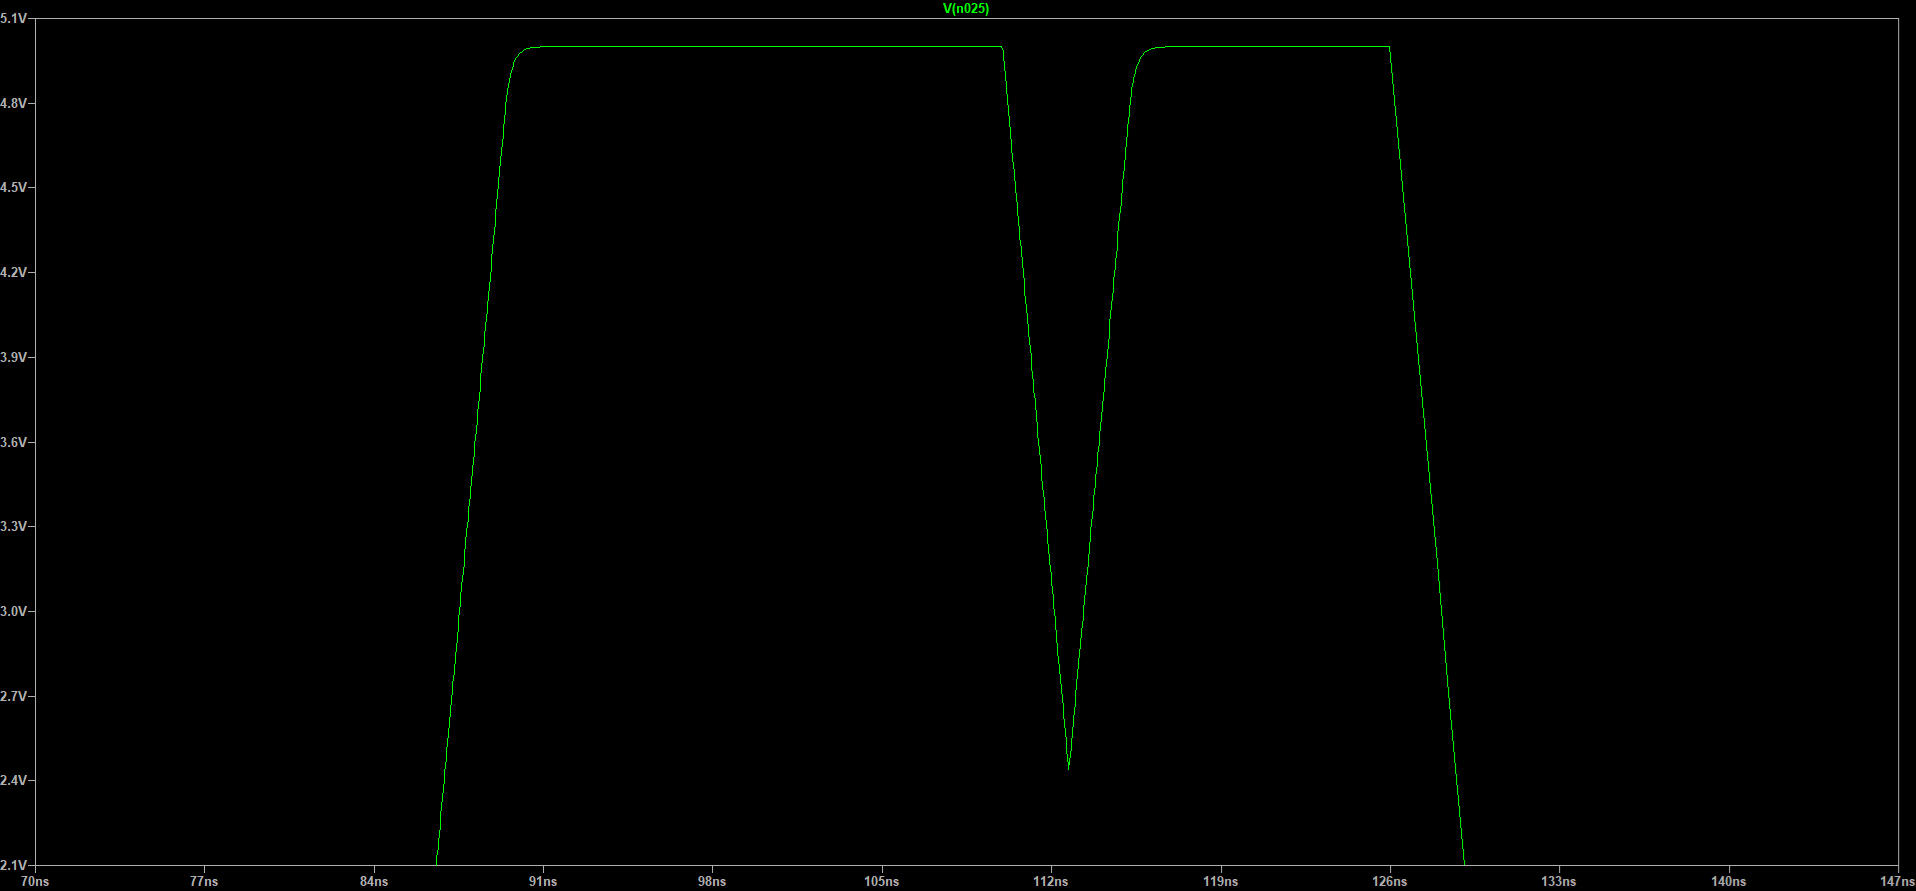
\includegraphics[width=1\textwidth]{popsute1.png}
    \end{adjustbox}
    \caption{Spadek napięcia z 5V do około 2.4V}
    \label{fig:mojobrazek}
\end{figure}

\begin{figure}[ht]
    \centering
    \begin{adjustbox}{center}
        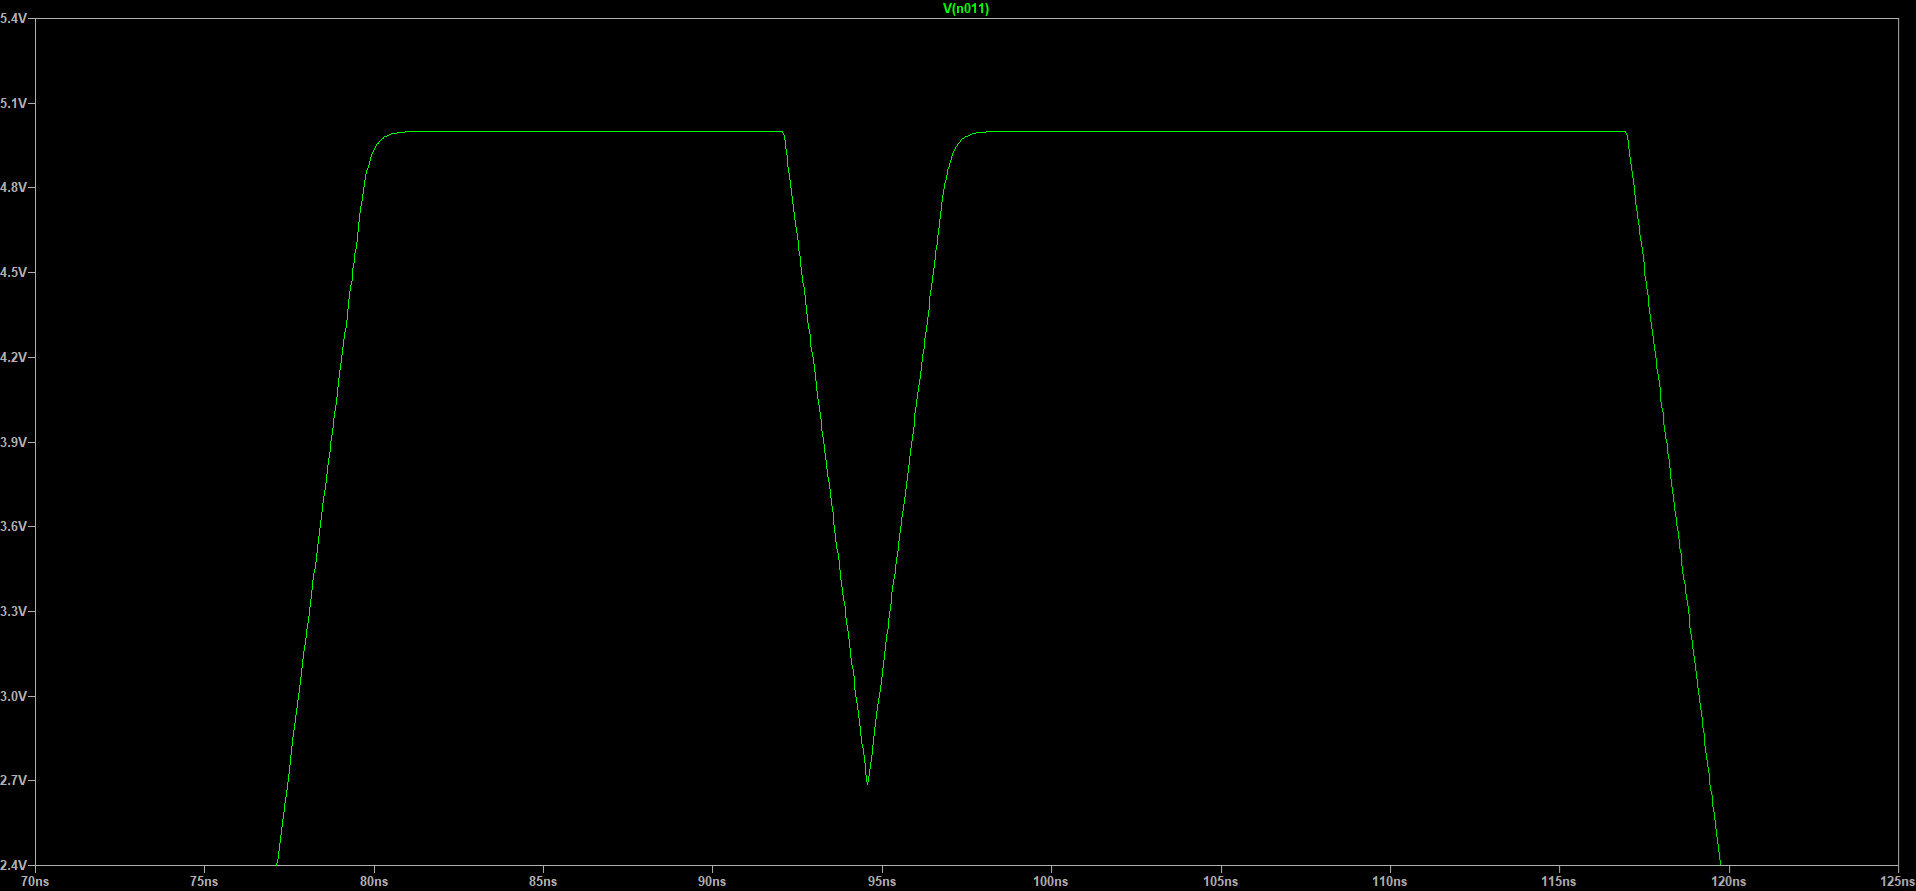
\includegraphics[width=1\textwidth]{popsute2.png}
    \end{adjustbox}
    \caption{Spadek napięcia z 5V do około 2.7V}
    \label{fig:mojobrazek}
\end{figure}

%%%%%%%%%%%%%%%%%%%%%
%6. Podsumowanie
%%%%%%%%%%%%%%%%%%%%%
\newpage
\section{Podsumowanie}
\subsection {Elementy idealne}
Symulacja na elementach idealnych dostarcza podstawowych danych na temat teoretycznego funkcjonowania kodera. Ze względu na brak ograniczeń fizycznych, takich jak opóźnienia lub rezystancja wewnętrzna, modele idealne pozwalają na przeprowadzenie symulacji w uproszczonej formie. Wyniki tej symulacji zapewniają czyste i klarowne dane wyjściowe, które zakrzywiają rzeczywiste działanie układu. Są one użyteczne głównie do wstępnych testów logicznych struktury kodera, pozwalając na identyfikację ewentualnych błędów logicznych w projektowaniu bez zakłóceń wynikających z fizycznych właściwości elementów.
\subsection {Elementy rzeczywiste}
Symulacja na elementach rzeczywistych jest znacznie bardziej kompleksowa. Wprowadzenie modeli, które uwzględniają czasy narastania i opadania sygnału, oporność, pojemność oraz inne realne charakterystyki elementów, pozwala na dokładniejsze odwzorowanie rzeczywistego działania układu. Takie symulacje są kluczowe do testowania układu w warunkach, które będą występować w praktycznych zastosowaniach, umożliwiając identyfikację potencjalnych problemów technicznych, takich jak problemy z czasowaniem, interferencje czy błędy wynikające z opóźnień sygnałów. Symulacja ta pozwala również na optymalizację projektu pod kątem wydajności i niezawodności, co jest niezbędne przed finalną realizacją projektu.
\subsection {Całokształt}
Analiza obu typów symulacji jest niezbędna dla kompleksowego rozwoju i weryfikacji układów elektronicznych. Symulacje na elementach idealnych oferują prostotę, która jest użyteczna w początkowych etapach projektowania, podczas gdy symulacje na elementach rzeczywistych dostarczają głębszego wglądu w działanie układu w realnych warunkach. Połączenie obu podejść pozwala na bardziej efektywne projektowanie, testowanie i implementację układów elektronicznych, co finalnie przekłada się na większą niezawodność i funkcjonalność finalnego produktu.

%%%%%%%%%%%%%%%%%%%%%
%6. Wnioski koncowe
%%%%%%%%%%%%%%%%%%%%%
\newpage
\section{Wnioski końcowe}
\begin{itemize}
    \item \textbf{Wyzwania w poszukiwaniu informacji}:
    Poszukiwanie informacji niezbędnych do realizacji zaawansowanych układów elektronicznych w sieci często nie przynosi oczekiwanych rezultatów. Wiele kluczowych danych na temat zaawansowanych technologii pozostaje niejawnych, a korporacje rzadko udostępniają informacje dotyczące swoich wysokobudżetowych projektów. Taki stan rzeczy znacząco utrudnia dostęp do pełnych, niezbędnych zasobów wiedzy, co stawia dodatkowe bariery w procesie naukowym i inżynierskim.
    \item \textbf{Projektowanie układu na elementach idealnych}:
    Realizacja projektu z wykorzystaniem elementów idealnych napotkała na przeszkody wynikające z braku dostępu do wystarczających informacji kluczowych do prawidłowego odtworzenia układu. Dopiero uzyskanie dostępu do schematów logicznych, które umożliwiły zastosowanie metody siatek Karnaugh do projektowania, pozwoliło na efektywne skonstruowanie układu idealnego w LTSpice. Ten etap podkreślił znaczenie posiadania konkretnych, szczegółowych danych dla osiągnięcia wiarygodnych wyników symulacji.
    \item \textbf{Implementacja układu z elementami rzeczywistymi}:
    Realizacja projektu z wykorzystaniem elementów rzeczywistych również napotkała bariery, głównie z powodu braku dostępnych modeli tych elementów w bibliotekach LTSpice. Sytuację udało się rozwiązać poprzez odnalezienie odpowiednich modeli na amatorskiej stronie internetowej, co umożliwiło kontynuację prac nad projektem. Ten przypadek dodatkowo podkreśla, jak kluczowe jest posiadanie dostępu do odpowiednich zasobów informacyjnych dla efektywnej realizacji projektów inżynierskich.
    \item \textbf{Edukacyjne i praktyczne korzyści}:
    Realizacja tego projektu przyniosła znaczne korzyści edukacyjne i praktyczne. Użytkowanie środowiska LTSpice w znaczny sposób poszerzyło nasze umiejętności praktyczne oraz utrwaliło wiedzę z zakresu techniki cyfrowej. Projekt ten uświadomił również, jak cenne i trudno dostępne są informacje dotyczące zaawansowanych rozwiązań technologicznych oraz projektów w dziedzinie elektroniki.
\end{itemize}

\newpage

\begin{thebibliography}{99}

\bibitem{ieee802} IEEE Standard Association, "IEEE 802.3-2015 - Standard for Ethernet," IEEE, 2015. [Online]. Adres: \url{https://ieeexplore.ieee.org/document/7428776} [Dostęp: 18-Kwie-2024].
\bibitem{opal} A. Opal, "Ethernet," Akademia Górniczo-Hutnicza w Krakowie. [Online]. Adres: \url{https://home.agh.edu.pl/~opal/sieci/wyklady/4-ethernet.pdf} [Dostęp: 18-Kwie-2024].
\bibitem{patent} M. Mazzola, L. Cafiero, and M. DeNicolo, "Method and apparatus for multilevel encoding for a local area network," U.S. Patent US 5280500A, Jan. 18, 1994. [Online]. Adres: \url{https://patents.google.com/patent/US5280500} [Dostęp: 18-Kwie-2024].
\bibitem{networkencyclopedia} Editorial Team, "100BaseTX: Implementation and Troubleshooting," Network Encyclopedia, Feb. 4, 2024. [Online]. Adres: \url{https://networkencyclopedia.com/100basetx/} [Dostęp: 18-Kwie-2024].
\bibitem{actel} Actel Corporation, "Using Actel FPGAs to Implement the 100 Mbit/s Ethernet Standard," April 1996. [Online]. Adres: \url{https://www.microsemi.com/document-portal/doc_view/129803-100mbethernet-an} [Dostęp: 09-Maj-2024].
\bibitem{ltwiki} Współautorzy LTwiki, "Main Page - LTwiki-Wiki for LTspice," Styczeń 17, 2024. [Online]. Adres: \url{https://ltwiki.org/index.php?title=Main_Page} [Dostęp: 10-Cze-2024].
\bibitem{borod} Bordodynov, "Bordodynov's Electronics Web Page" 2024 [Online]. Adres: \url{http://bordodynov.ltwiki.org/} [Dostęp: 11-Cze-2024].
\bibitem{hc04} Diodes Incorporated, "74HC04 Datasheet," Diodes, [Online]. Adres: \url{https://www.diodes.com/assets/Datasheets/74HC04.pdf} [Dostęp: 12-Cze-2024].
\bibitem{hc08} Diodes Incorporated, "74HC08 Datasheet," Diodes, [Online]. Adres: \url{https://www.diodes.com/assets/Datasheets/74HC08.pdf} [Dostęp: 12-Cze-2024].
\bibitem{hc32} Diodes Incorporated, "74HC32 Datasheet," Diodes, [Online]. Adres: \url{https://www.diodes.com/assets/Datasheets/74HC32.pdf} [Dostęp: 12-Cze-2024].
\bibitem{hc11} Texas Instruments, "CD74HC11 Datasheet," Texas Instruments, [Online]. Adres: \url{https://www.ti.com/lit/ds/symlink/cd74hc11.pdf} [Dostęp: 12-Cze-2024].

\end{thebibliography}

\newpage
\listoffigures
\listoftables

\end{document}